\documentclass[10pt]{article}

% --- Packages ---
\usepackage[utf8]{inputenc}    % Standard encoding
\usepackage[margin=1in]{geometry} % Page margins
\usepackage{graphicx}          % For including images
\usepackage{amsmath, amssymb}  % Essential math symbols
\usepackage{booktabs}          % Professional quality tables
\usepackage{float}
\usepackage[backend=biber, style=ieee]{biblatex}
\addbibresource{references.bib}
\setlength{\abovecaptionskip}{-2pt}

\begin{document}

% --- Custom Full-Width Title Block ---
%\twocolumn[{%
  \begin{center}
    {\LARGE \textbf{Project 2: Extracting Images and Displacements from Raw Spectral Domain Optical Coherence Tomography Data} \par}
    \vspace{0.4cm}
    
    {\Large Sophia Klymchuk \par}
    \vspace{0.2cm}
    
    {\large \textit{ECE-435: Medical Imaging} \par}
    {\large Prof. Brian Frost \par}
    \vspace{0.4cm}
    
    {\large April 8, 2026 \par}
    \vspace{0.8cm} % Adds space before the columns start
  \end{center}
%}]


\begin{abstract}
This project explores the fundamental principles of medical image reconstruction and processing using a thoracic CT dataset. Methods explored include slicing, various types of filtering for noise reduction, and edge detection techniques.
\end{abstract} 

\section{Introduction}
Optical coherence tomography (OCT) is a biomedical imaging modality that produces volumetric, depth-resolved images with micron-scale resolution using only light. OCT is powerful because it can noninvasively visualizes tissue microstructure and pathology without the need for physical excision \cite{fujimotoIntroductionOCT2015}.

OCT employs low-coherence interferometry to measure sample reflectivity as a function of depth, without physical contact or sectioning \cite{izattTheoryOpticalCoherence2015}. Of the three primary OCT paradigms---time-domain, spectral-domain, and swept-source---spectral-domain OCT (SD-OCT) offers a significant signal-to-noise advantage by capturing all depth information simultaneously on a detector array rather than scanning sequentially \cite{izattTheoryOpticalCoherence2015}.

In SD-OCT, a broadband near-infrared source illuminates a Michelson-style interferometer that splits light between a reference arm and a sample arm, each a distance $z_R$ and $z_S$, respectively, from the beam splitter. The travelled path of light is assumed to be in air, which has an index of refraction $n=1$. When split, $a_R$ and $a_S$ are unitless values that represent the proportion of amplitude split between the reference and sample beams, respectively. After reflecting off of either the sample or the reference mirror (which has reflectivity $r_R$), the sample and reference beams, respectively, recombine and are dispersed by a diffraction grating onto a line camera, where each pixel records the intensity of a different optical wavelength $\lambda$. The resulting wavelength-domain intensity pattern encodes the depth-resolved reflectivity profile of the sample in its spectral frequency content \cite{izattTheoryOpticalCoherence2015,brianlfrostthesis}. 

In deriving the model for SD-OCT, we utilize the wavenumber, defined as $k=\frac{2\pi}{\lambda}$, as well as the spectral intensity $S(k) =< |s(k) e^{j\omega t} |^2 >$ (where $s(k)$ is the electric field spectrum, and $<\cdot>$ is integration over photodetector measuring time). The measured intensity can be defined, as a function of wavenumber $k$:

\begin{equation}
\begin{split}
I^D(k) &= \frac{\rho}{2} S(k) \left( a_R^2 r_R^2 + a_S^2 \sum_{m=1}^M r_m^2 \right) \\
&\quad + \frac{\rho}{2} S(k) a_R a_S r_R \sum_{m=1}^M \left( r_m \left( e^{j2k(nz_m-z_R)} + e^{j2k(z_R-nz_m)} \right) \right) \\
&\quad + \frac{\rho}{2} S(k) \sum_{l \neq m} \{ r_l r_m \left( e^{j2kn(z_l-z_m)} + e^{j2kn(z_m-z_l)} \right) \}
\end{split}
\label{eq:k_intensity}
\end{equation}

In Equation~\ref{eq:k_intensity}, the sample is modeled as a stack of $M$ point reflectors, with each reflector at a physical depth of $z_m$ into the sample with reflectivity $r_m$, for $m$ ranging from $1$ to $M$. Here, the first term is independent of $z$, representing a DC component that scales the source spectrum. The second and third terms, respectively, represent cross- and auto-correlation between reference and sample beams, or various sample reflector beams.

Utilizing Euler's identity on the exponential terms, as well as ignoring the autocorrelation terms due to assumptions of a perfectly reflecting mirror ($r_R \approx 1$) and small layer-by-layer point reflectivities in the sample ($r_m<<1$), we get:

\begin{equation}
\begin{split}
  I^D(k) \approx GS(k) + HS(k)\sum_{m=1}^M \left( r_m \cos\left( 2k \left( nz_m-z_R\right)\right) \right) \\
  G = \frac{\rho}{2}\left(a_R^2r_R^2 + a_S^2 \sum_{m=1}^{M}r_m^2\right), \quad H=\rho a_R a_S r_R
\end{split}
\label{eq:compact_k_intensity}
\end{equation}

Note that because the OCT signal modeled by Equation~\ref{eq:compact_k_intensity} encodes the depth of each reflector in the spatial-frequency domain, the fundamental processing step is an inverse Fourier transform of this signal. This Fourier-transformed signal yields an A-scan: a one-dimensional map of reflectivity along the depth of the beam axis (in the space domain).

Before transforming the OCT signal to the space domain, we can subtract the DC term $GS(k)$, a step termed background subtraction. The DC term is estimated by blocking the sample beam to obtain $S(k)$, while $G$ is estimated from the average value of the OCT signal. Dividing the result by $S(k)$ then performs spectral normalization, which is equivalent to deconvolution in the spatial domain by the Fourier transform of the source spectrum.

Because the raw OCT signal is real-valued, the Fourier-transformed space domain A-scan will be conjugate-symmetric with respect to depth (where values are reflected across the origin). Thus, after taking the Fourier transform of the OCT signal, we can only consider positive depth without losing any information.

This report details the complete processing pipeline for raw SD-OCT data acquired on a ThorLabs Telesto~3 system. Three datasets are processed: a B-scan (a laterally-sampled collection of A-scans forming a cross-sectional image) of a stack of Scotch tape layers, and two M-scans (time series of A-scans at a fixed lateral position) acquired near a speaker membrane while it played a single tone and a 40-tone complex, respectively, at 80~dB sound pressure level (SPL). The M-scans are acquired with a sampling rate of $f_{s}$, resulting in a temporal spacing of $\Delta t=1/f_{s}$ between consecutive A-scans. Processing goals include construction of the B-scan image and extraction of sub-pixel displacement measurements from the M-scans via spectral domain phase microscopy (SDPM).

The system uses a superluminescent diode (SLD) source with center wavelength $\lambda_0 \approx 1300$~nm and bandwidth $\Delta\lambda \approx 100$~nm. A-scans are recorded over $N = 2048$ charge-coupled device (CCD) pixels with an axial pixel size of $dz = 3.6$~\textmu m. The LSM-03 objective lens has numerical aperture $\mathrm{NA} = 0.055$. In each dataset, the first $D$ columns contain background samples acquired by blocking the sample beam; these are used for background subtraction and deconvolution in processing.

\section{Guiding Computations}

\subsection{Lateral Resolution}
The lateral resolution of an SD-OCT system is governed by the focusing geometry---specifically the central wavelength and the numerical aperture of the objective lens. At the focal plane, the lateral resolution is given by the full width at half maximum (FWHM) of the confocal point spread function \cite{izattTheoryOpticalCoherence2015, brianlfrostthesis}:
\begin{equation}
  \delta x = \delta y \approx 0.37 \frac{\lambda_0}{\mathrm{NA}}
  \label{eq:lateral_resolution}
\end{equation}
Note that at depths away from the focal plane, the lateral resolution degrades as the beam diverges. Given $\lambda_0 \approx 1300$~nm and $\mathrm{NA} = 0.055$, the expected lateral resolution is $\delta x \approx 8.75$~\textmu m.

\subsection{Axial Resolution}
The axial resolution of an SD-OCT system is decoupled from the lateral resolution and is instead determined by the coherence length of the light source \cite{izattTheoryOpticalCoherence2015}. For a Gaussian-shaped source spectrum, the axial resolution (FWHM of the coherence function) is given by:
\begin{equation}
  \delta z = \frac{2 \ln 2}{n \pi}\frac{\lambda_0^2}{\Delta\lambda}
  \label{eq:axial_resolution}
\end{equation}
Given $\lambda_0 \approx 1300$~nm and $\Delta\lambda \approx 100$~nm, the expected axial resolution is $\delta z \approx 7.46$~\textmu m.

The axial pixel size ($dz = 3.6$~\textmu m) is finer than the axial resolution ($\delta z = 7.46$~\textmu m); the two are distinct quantities. The pixel size sets the sampling interval in the depth domain, while the resolution sets the minimum separation at which two reflectors can be distinguished.

\subsection{B-Scan Pixel Aspect Ratio}
Two related quantities are relevant: the pixel aspect ratio (the physical shape of a single pixel) and the image aspect ratio (the physical dimensions of the full B-scan).

The axial pixel size is $dz = 3.6$~\textmu m. The B-scan contains $M = 10{,}000$ A-scans spanning 1~mm, giving a lateral pixel size of:
\begin{equation*}
  dx = \frac{1\;\text{mm}}{10{,}000} = 0.1\;\mu\text{m}
\end{equation*}
The pixel aspect ratio is therefore:
\begin{equation*}
  \frac{dx}{dz} = \frac{0.1\;\mu\text{m}}{3.6\;\mu\text{m}} = \frac{1}{36}
\end{equation*}
Since this ratio is less than one, each pixel is taller than it is wide. Displaying the image with square pixels would compress structures laterally relative to their true proportions. The correct display approach sets \texttt{extent} in physical units (mm) and uses \texttt{aspect="equal"} in \texttt{imshow}.

For the image aspect ratio, the B-scan width is fixed at 1~mm. The axial extent depends on whether the mirror-image artifact is retained. Because the OCT signal is real-valued, its Fourier transform is conjugate-symmetric: the A-scan contains a true depth profile at positive depths and a redundant mirror image at negative depths \cite{izattTheoryOpticalCoherence2015}. Retaining both halves yields $2048 \times 3.6\;\mu\text{m} = 7.37$~mm of depth, giving a width-to-height ratio of approximately $1{:}7.4$. After discarding the mirror half, the depth reduces to $1024 \times 3.6\;\mu\text{m} = 3.69$~mm, giving a ratio of approximately $1{:}3.7$. Only the mirror-cropped image is used for display and analysis.


\section{Methodology}

\subsection{A-Scan Processing Pipeline}
The raw SD-OCT data consists of electron counts on each of the $N = 2048$ CCD pixels for every A-scan. These counts represent the wavelength-domain OCT signal, sampled approximately linearly in wavelength and therefore nonlinearly in wavenumber. The processing pipeline converts this raw signal into a complex-valued, depth-resolved A-scan through five steps: (1)~background subtraction, (2)~windowing, (3)~deconvolution, (4)~wavelength-to-wavenumber (L2K) resampling, and (5)~Fourier transformation.

Each dataset includes a set of background A-scans (acquired with the sample beam blocked) at the beginning of the file: 175 for the B-scan and 320 for each M-scan. These background scans are used in both the subtraction and deconvolution steps.

The raw OCT signal contains a large DC component from the reference beam intensity and the average sample reflectivity (see Equation~\ref{eq:compact_k_intensity}), neither of which encodes depth-resolved information \cite{izattTheoryOpticalCoherence2015,brianlfrostthesis}. If left unremoved, this DC term produces a large artifactual spike at zero depth that can overwhelm nearby true reflector signals. The autocorrelation terms arising from pairwise interference among sample reflectors also cluster near zero depth \cite{izattTheoryOpticalCoherence2015}.

To remove the DC component, the averaged background spectrum is subtracted from each signal A-scan \cite{brianlfrostthesis}. The raw (unsmoothed) average of the background scans is used for this subtraction to avoid introducing smoothing artifacts.

After background subtraction, a Hanning window is applied in the wavenumber domain. Windowing suppresses spectral leakage that would otherwise arise from the abrupt truncation of the signal at the detector edges \cite{brianlfrostthesis}.

Even after background subtraction, the depth-domain point spread function remains shaped by the source spectrum $S(k)$. Deconvolution compensates for this by dividing the background-subtracted signal by $S(k)$ in the wavenumber domain, which is equivalent to deblurring by the PSF in the spatial domain.

Dividing by the raw (noisy) background spectrum would amplify noise at wavenumbers where the source power is low. Instead, a polynomial is fit to the averaged background spectrum, and the resulting smooth curve serves as the denominator. The polynomial order was chosen by visually comparing the fit to the averaged background.

Because the spectrometer data is recorded via array camera in the wavelength domain, but the Fourier transform step requires sampling that is linear in wavenumber, the signal is resampled from wavelength to wavenumber space (L2K resampling) using linear interpolation \cite{brianlfrostthesis}. This was done via a matrix multiplication approach, where the resampling matrix was given as a precomputed constant, based on the experimental setup.

After background subtraction, windowing, deconvolution, and L2K resampling, the inverse Fourier transform is applied along the wavenumber axis. Because the OCT signal is real-valued, the transform is conjugate-symmetric; only the positive-depth half is retained, discarding the mirror image. The resulting complex-valued A-scan encodes reflectivity in its magnitude and sub-pixel displacement information in its phase (used later for SDPM). The magnitude is displayed in dB as $20\log_{10}|A(z)|$.

\subsection{B-Scan Formation}
The B-scan function extends the A-scan processing to the full dataset, avoiding redundant computation. In the A-scan pipeline, certain operations — specifically, computing the average background and its polynomial fit — depend only on the background columns and are identical for every A-scan in the B-scan. These computations need only be performed once. The windowing function and the smoothed background for deconvolution are similarly fixed across A-scans. The B-scan function should therefore precompute these quantities once and then apply them simultaneously to all M signal A-scans as a single operation.

After processing, the result is a complex-valued $N/2 \times M$ matrix (retaining only the positive-depth half after discarding the mirror image). The magnitude of this matrix, expressed in dB, constitutes the raw B-scan image.

Contrast enhancement was necessary after producing the B-scan image, as the raw dB-magnitude image spanned a very large dynamic range. The A-scan magnitudes were examined first to identify the useful dynamic range in order to set appropriate dB thresholds for grayscale display. 


\subsection{M-Scan and Spectral Domain Phase Microscopy}

Spectral domain phase microscopy (SDPM) exploits the phase of the complex A-scan (rather than its magnitude) to measure sub-pixel displacements of reflectors along the beam axis. The phase of the complex A-scan at pixel $z_0$ is related to the displacement $d(t)$ of the reflector at that depth by Equation~\ref{eq:sdpm_displacement}, where $\lambda_0$ is the central wavelength of the source, $n$ is the index of refraction of the medium, and $\phi(z_0, t)$ is the temporally-varying phase of the complex A-scan at depth $z_0$ \cite{brianlfrostthesis}.

\begin{equation}
d(t) = \frac{\lambda_0 \, \phi(z_0, t)}{4\pi n}
\label{eq:sdpm_displacement}
\end{equation}

It should be noted that SDPM only measures the projection of three-dimensional motion onto the OCT beam axis. If the true displacement is not purely along the beam axis, the measured displacement will underestimate the full magnitude; this is an inherent limitation of uniaxial OCT-based vibrometry \cite{brianlfrostthesis}.

Given the complex M-scan $A(z, t)$ computed by applying a A-scan processing pipeline to each time sample, SDPM proceeds as follows:
\begin{enumerate}
  \item Select the pixel of interest: Identify depth index $z_0$ corresponding to the reflector to be tracked (e.g., the speaker membrane surface), identified from the average A-scan magnitude as a peak of high intensity.
  \item Extract the phase time series: Compute $\phi(z_0, t) = \angle(A(z_0, t))$ for all time samples. This raw phase will be wrapped to $[-\pi, \pi]$.
  \item Unwrap the phase: Apply phase unwrapping along the time axis to remove $2\pi$ discontinuities, yielding a continuous phase signal. This is essential because the true displacement may accumulate phase beyond $\pm \pi$ between consecutive samples.
  \item Convert phase to displacement: Apply Equation~\ref{eq:sdpm_displacement} to obtain $d(t)$ in physical units (mm).
  \item Frequency-domain analysis: Take the Fourier transform of $d(t)$, using the sampling interval $\Delta t = \frac{1}{f_s}$, to obtain the displacement spectrum. Peaks in this spectrum identify the frequencies of vibration.
\end{enumerate}

It should be noted that a large transient artifact was observed at the beginning of the M-scan datasets, likely due to the onset of speaker vibration. To avoid this artifact, the first 100 time samples were discarded from pixel $z_0$ candidates. Additionally, a steady linear drift was observed in the raw time series, which was removed via \texttt{scipy.signal.detrend} before further analysis.

For the M-scans, the average A-scan magnitude was  computed first to identify the depth of the speaker membrane as a band of high intensity. Two high-intensity pixels at this depth were selected for tracking in both time and frequency domains.

\section{Results and Discussion}

\subsection{A-Scan Processing}
The averaged background scans and sample polynomial fittings are shown in Appendix \ref{appendix:poly_fitting}, where it was demonstrated that a polynomial of degree $16$ was appropriate for smoothness and accuracy without numerical instability. This smooth polynomial estimate of the source spectrum $S(k)$ was used exclusively for deconvolution; the raw averaged background was used for the DC subtraction step.

Figure~\ref{fig:ascans_full} shows the magnitude (dB) of two A-scans from the B-scan dataset and one from each M-scan dataset, all processed with the full pipeline. The B-scan A-scans show a cluster of bright reflections between 
approximately $0.5$ and $1.5$ mm depth corresponding to the tape layers, with a noise floor near $-20$ dB. The two M-scan A-scans are similar to one another in structure, as 
expected, both are acquired at the same lateral location near the speaker membrane.


\begin{figure}[ht]
  \centering
  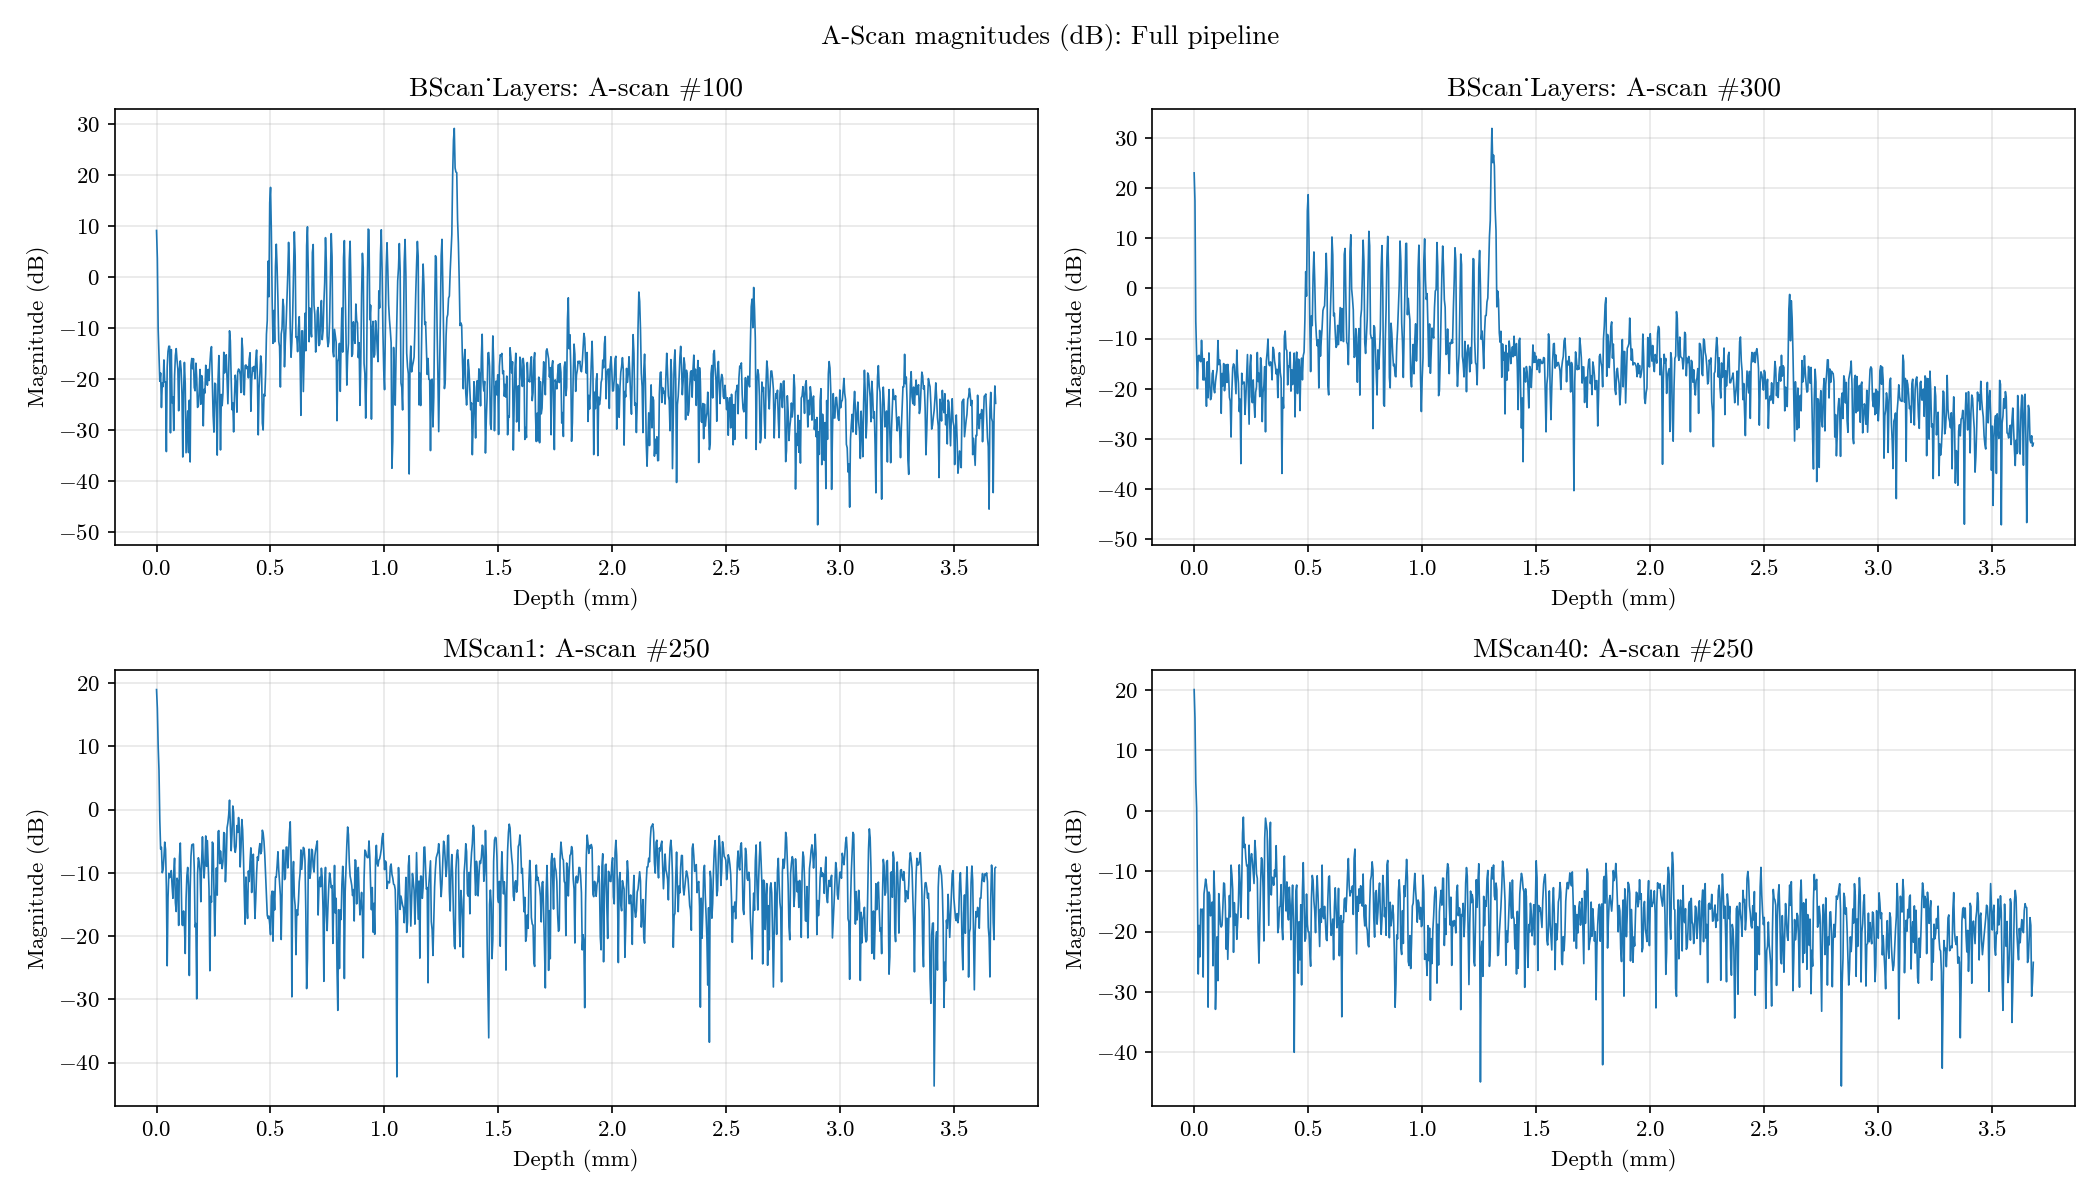
\includegraphics[width=\textwidth]{Results/ascans_full_pipeline.png}
  \caption{A-scan magnitudes (dB) from the full processing pipeline. Top left and top 
  right: two A-scans from the B-scan dataset. Bottom left: one A-scan from the 
  single-tone M-scan. Bottom right: one A-scan from the 40-tone M-scan. The 
  M-scan A-scans are closely similar in structure, as both are acquired at the same 
  location above the speaker membrane.}
  \label{fig:ascans_full}
\end{figure}



Figure~\ref{fig:pipeline_comparison} compares the same A-scan (taken from the B-scan dataset) processed under three conditions: the full pipeline (background subtraction, windowing, and deconvolution), background subtraction and windowing only (no deconvolution), and neither background subtraction nor deconvolution.

\begin{figure}[ht]
  \centering
  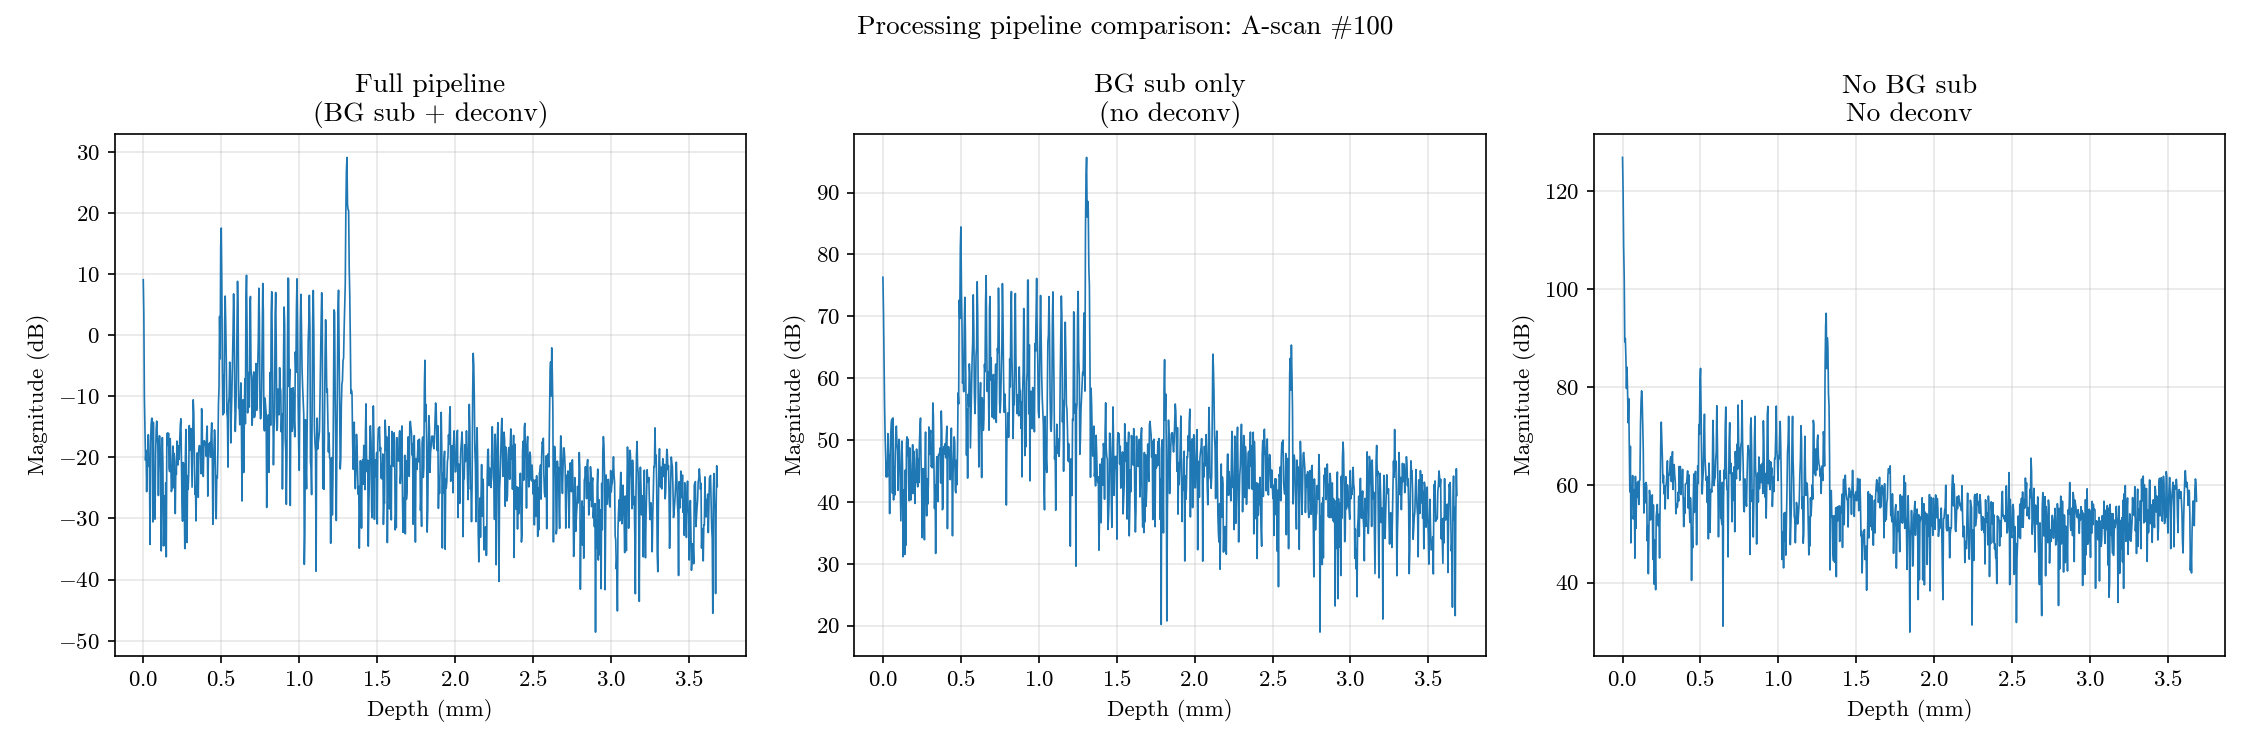
\includegraphics[width=\textwidth]{Results/pipeline_comparison.png}
  \caption{Pipeline comparison for A-scan \#100 from the B-scan dataset. Left: full pipeline. Center: background subtraction and windowing only, no deconvolution. Right: no background subtraction, no deconvolution.}
  \label{fig:pipeline_comparison}
\end{figure}

Without background subtraction, the large DC component of the reference dominates the signal near zero depth. After background subtraction alone, the DC spike is still present, but largely eliminated, and the tape layer reflections become clearly visible. Deconvolution does not appear to increase the interpretability of the peaks, as the raw A-scan already has a very high SNR. However, it does shift the magnitude of the signal downwards in magnitude, which may be the deconvolution normalizing the signal by the smoothed background spectrum. In cases where the SNR is lower at the start, deconvolution would be expected to improve the axial resolution by effectively dividing out $S(k)$ in the wavenumber domain.

\subsection{B-Scan Imaging}

To correctly pick magnitude limits for display, the A-scan magnitudes were examined to identify the useful dynamic range. The 10th and 99th percentiles of the A-scan magnitudes were used as the lower and upper limits, respectively, for contrast enhancement.

Figure~\ref{fig:bscan} shows the B-scan of the Scotch tape stack, unprocessed and contrast-enhanced.

\begin{figure}[ht]
  \centering
  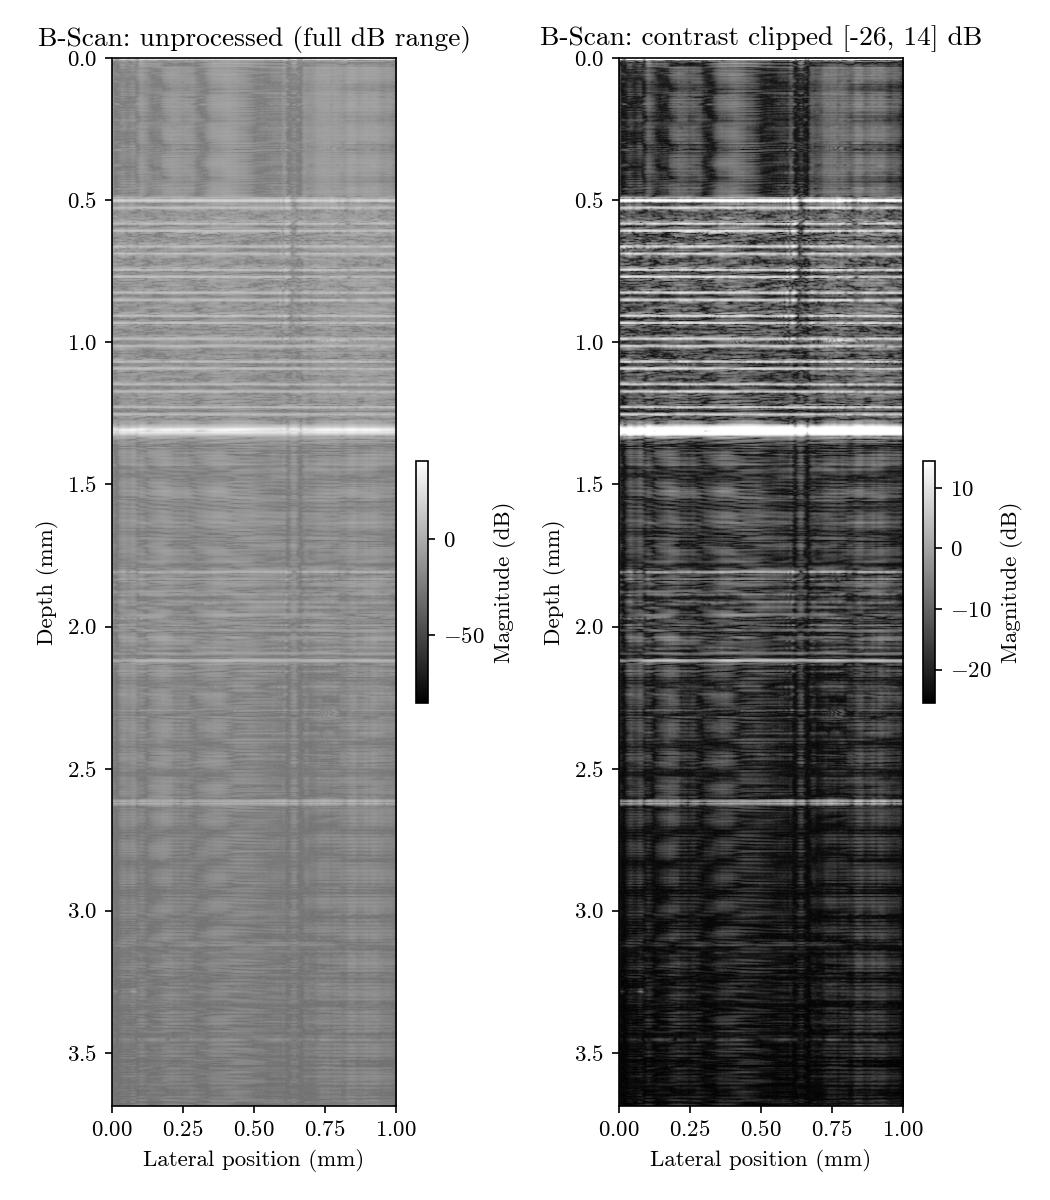
\includegraphics[width=0.5\textwidth]{Results/bscan_full_pipeline.png}
  \caption{B-scan of the Scotch tape stack (full processing pipeline). Left: raw dB image with no contrast clipping. Right: contrast-enhanced image with display range clipped to $[-26, 14]$~dB. Physical axes are shown in mm with correct aspect ratio ($1\,\text{mm}$ wide, $3.69\,\text{mm}$ deep after mirror removal).}
  \label{fig:bscan}
\end{figure}

The unprocessed image is dominated by the very high dynamic range of the raw OCT signal, a linear grayscale colormap applied over the full range renders the weaker structure invisible. Contrast was enhanced by clipping the display range to the interval $[-26, 14]$~dB corresponding to the 10th and 99th percentiles of the A-scan magnitudes. Signals below the lower threshold are rendered black; those above the upper threshold are rendered white. 

In the contrast-enhanced image, $10$ distinct bright bands are visible, corresponding to $10$ sheets of Scotch tape. There are also thinner bands visible between the thicker ones, which likely represent the air-tape interfaces in between each sheet of Scotch tape. The tape sheets are estimated to be about $0.05$ mm, while the separation bands in between are roughly $0.03$ mm.

Figure~\ref{fig:bscan_deconv} compares B-scans produced with and without deconvolution (both with background subtraction). Both images are constrast-enhanced with their respective 10th and 99th percentile dB ranges. As noted before when inspecting deconvolved vs. non-deconvolved A-scans, deconvolution does not appear to increase the interpretability of the B-scan image, as the raw signal already has a very high SNR. However, it does shift the magnitude of the signal downwards in magnitude, which is evident in the dB magnitude range of the images' colorbars. 

\begin{figure}[ht]
  \centering
  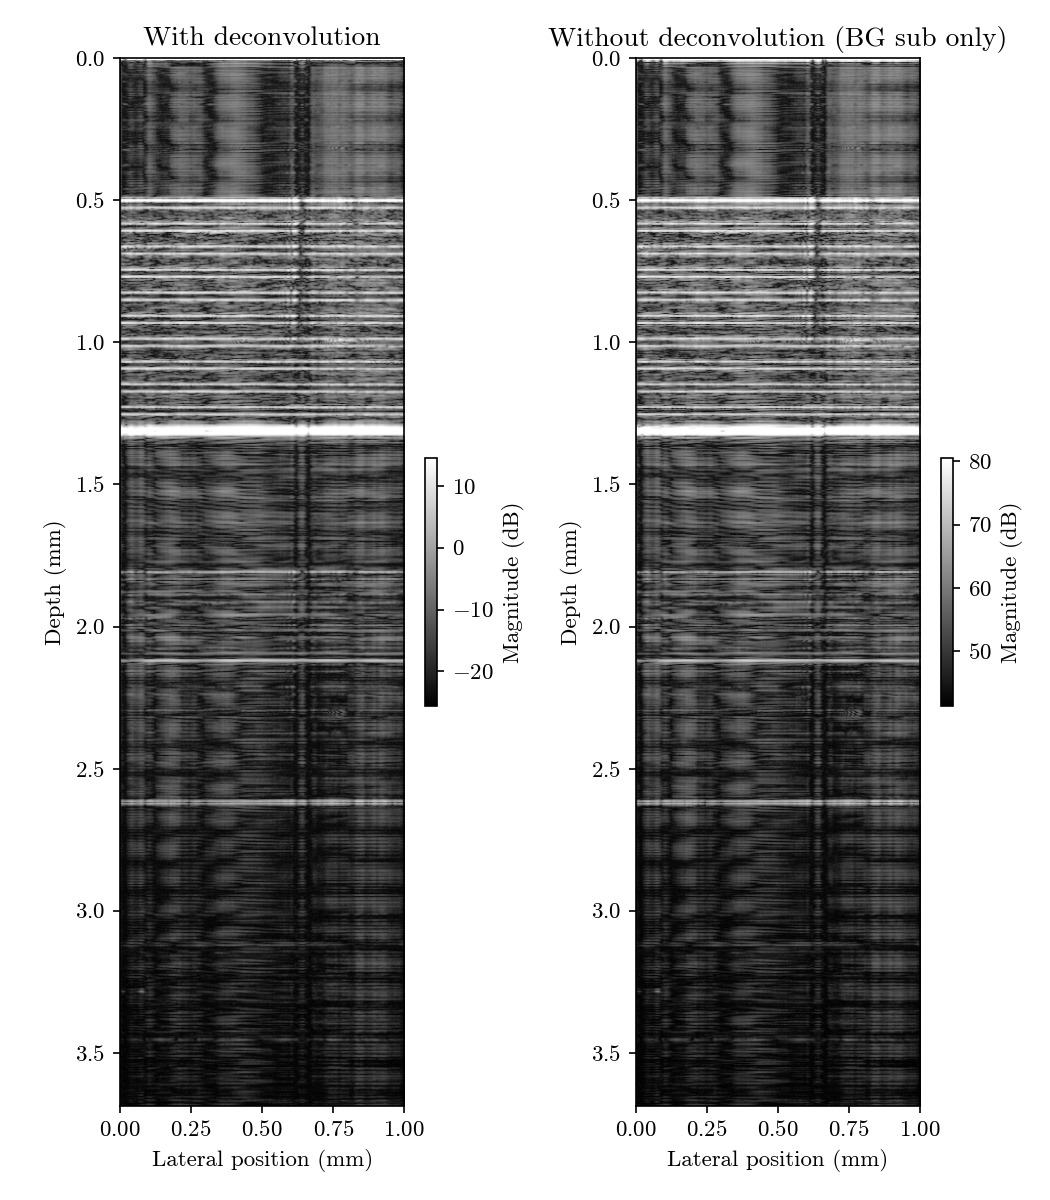
\includegraphics[width=0.5\textwidth]{Results/bscan_deconv_comparison.png}
  \caption{Effect of deconvolution on B-scan image quality. Left: full pipeline (with deconvolution). Right: background subtraction only, no deconvolution. Both images are contrast-enhanced using their respective 10th--99th percentile dB ranges.}
  \label{fig:bscan_deconv}
\end{figure}


\subsection{M-Scan and Spectral Domain Phase Microscopy}

\subsubsection{Single Tone M-Scan}

Figure~\ref{fig:mscan1_avg} shows the time-averaged A-scan magnitude for the single-tone M-scan. A prominent high-intensity band is visible near $0.25$~mm depth corresponding to the surface of the speaker membrane. Two tracking pixels were selected near this depth utilizing \texttt{scipy.signal.find\_peaks}: pixel A at index $60$ ($0.216$~mm) and pixel B at index $93$ ($0.335$~mm). These pixels are marked with red and blue 'x' markers, respectively, in the figure. Both pixels are located within the high-intensity band corresponding to the speaker membrane, making them suitable candidates for SDPM tracking of the membrane's vibration. The exact depth of the membrane is not precisely known, so selecting multiple pixels within this band allows for comparison of their SDPM results and ensures that at least one is accurately tracking the membrane surface.

\begin{figure}[ht]
  \centering
  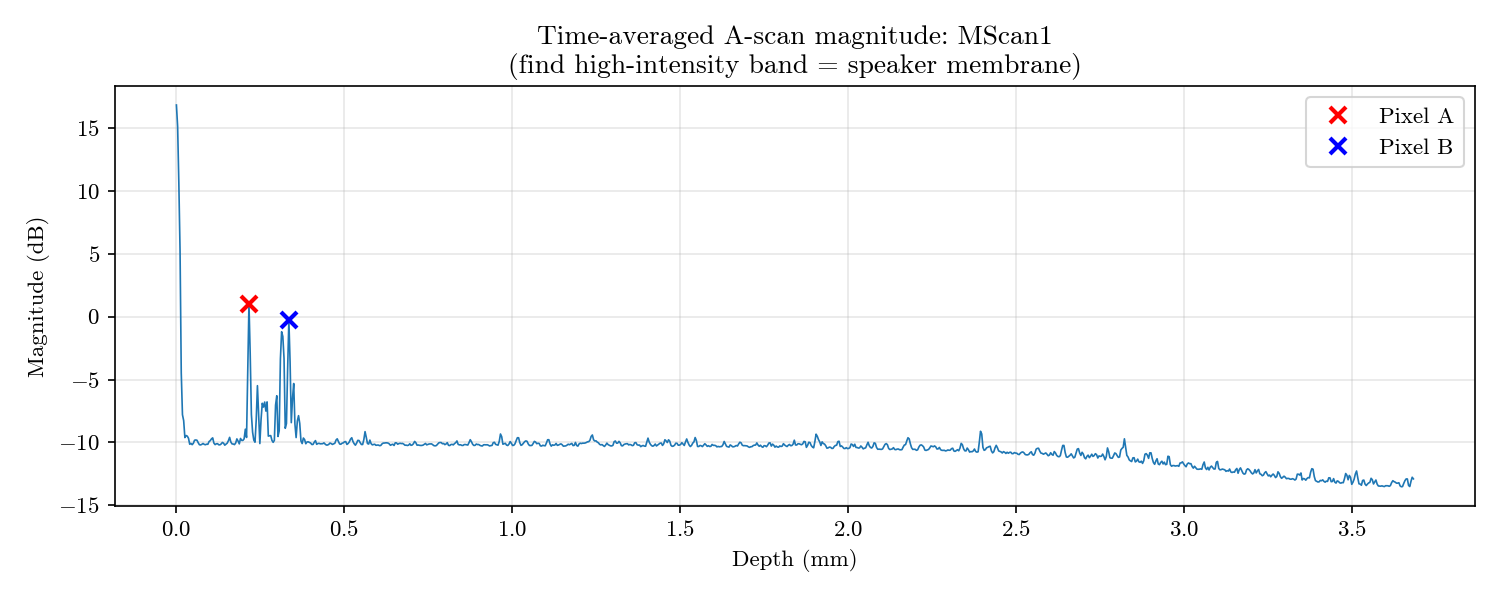
\includegraphics[width=\textwidth]{Results/mscan1_avg_magnitude.png}
  \caption{Time-averaged A-scan magnitude (dB) for the single-tone M-scan. The high-intensity band near $0.25$~mm identifies the speaker membrane. Pixels A (index $60$) and B (index $93$), marked with red and blue 'x' markers respectively, were selected for SDPM tracking.}
  \label{fig:mscan1_avg}
\end{figure}

Figures~\ref{fig:mscan1_A} and~\ref{fig:mscan1_B} show the time-domain displacement and frequency-domain spectrum for pixels A and B, respectively.

\begin{figure}[ht]
  \centering
  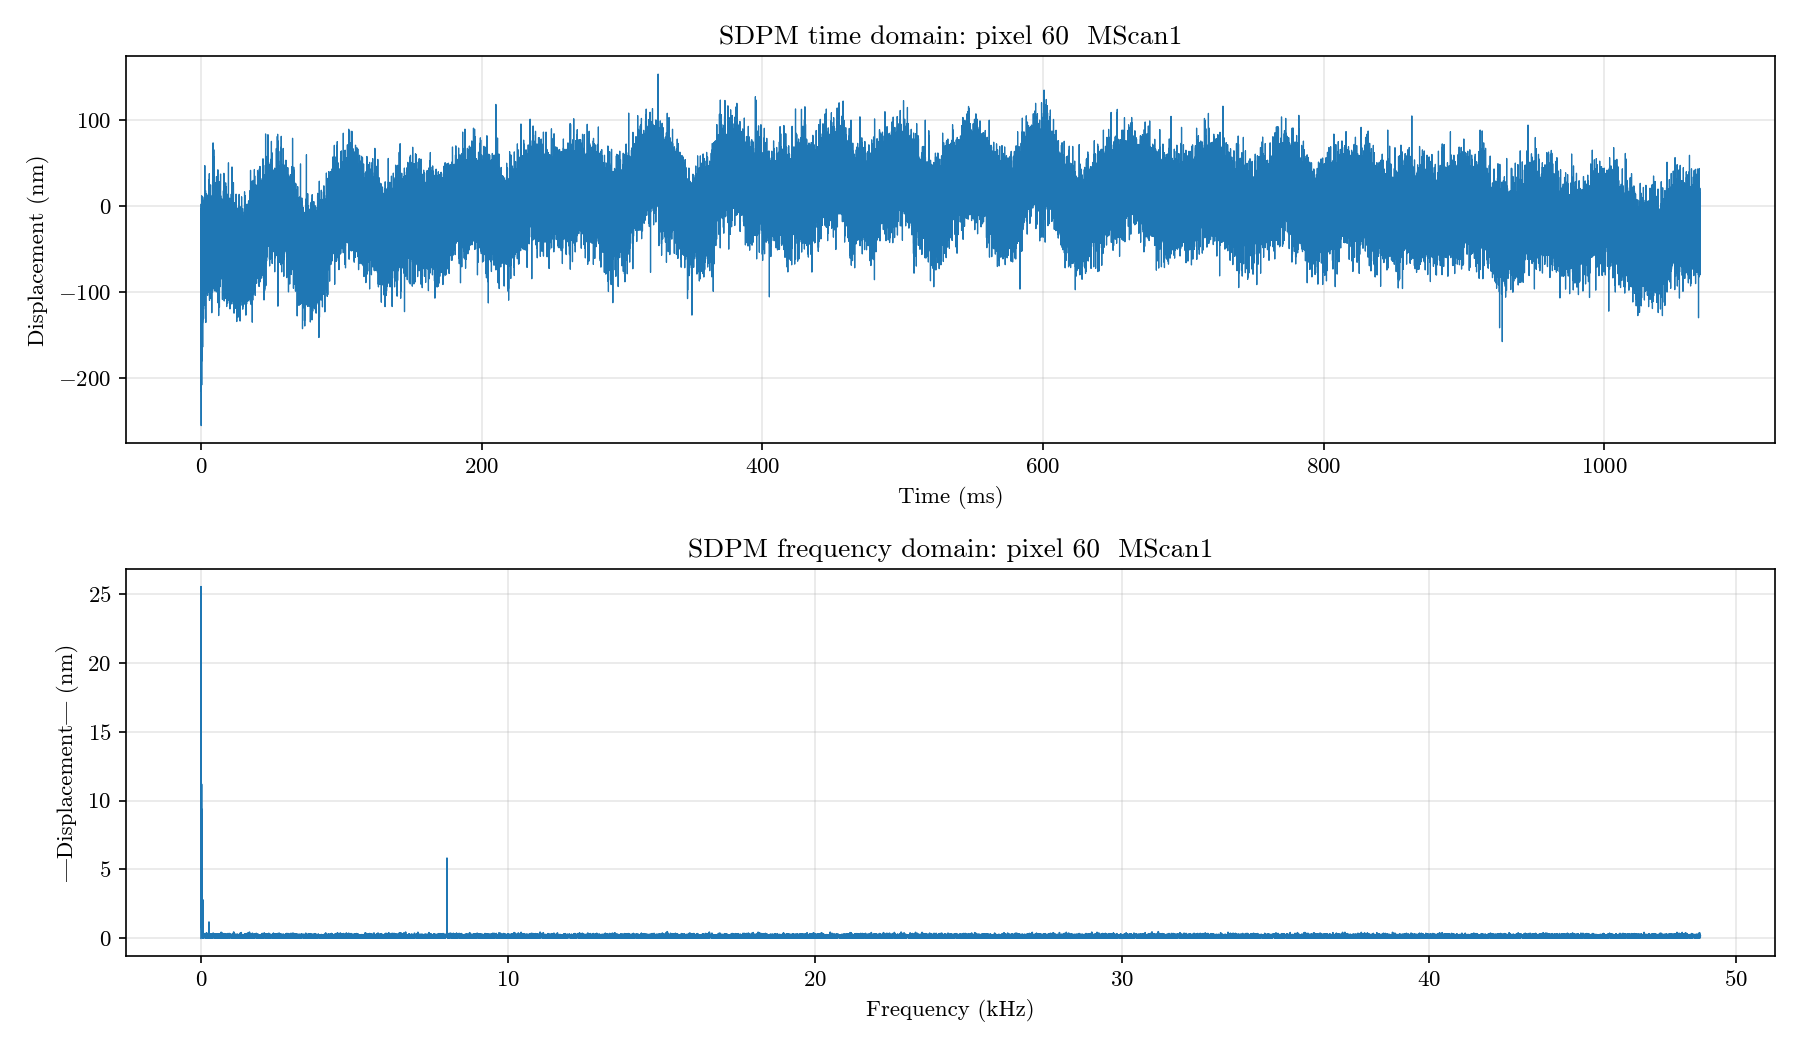
\includegraphics[width=\textwidth]{Results/mscan1_sdpm_pixelA.png}
  \caption{SDPM result for pixel A (index $60$, depth $0.216$~mm) in the single-tone M-scan. Top: displacement time series (nm). Bottom: one-sided displacement spectrum (nm).}
  \label{fig:mscan1_A}
\end{figure}

\begin{figure}[ht]
  \centering
  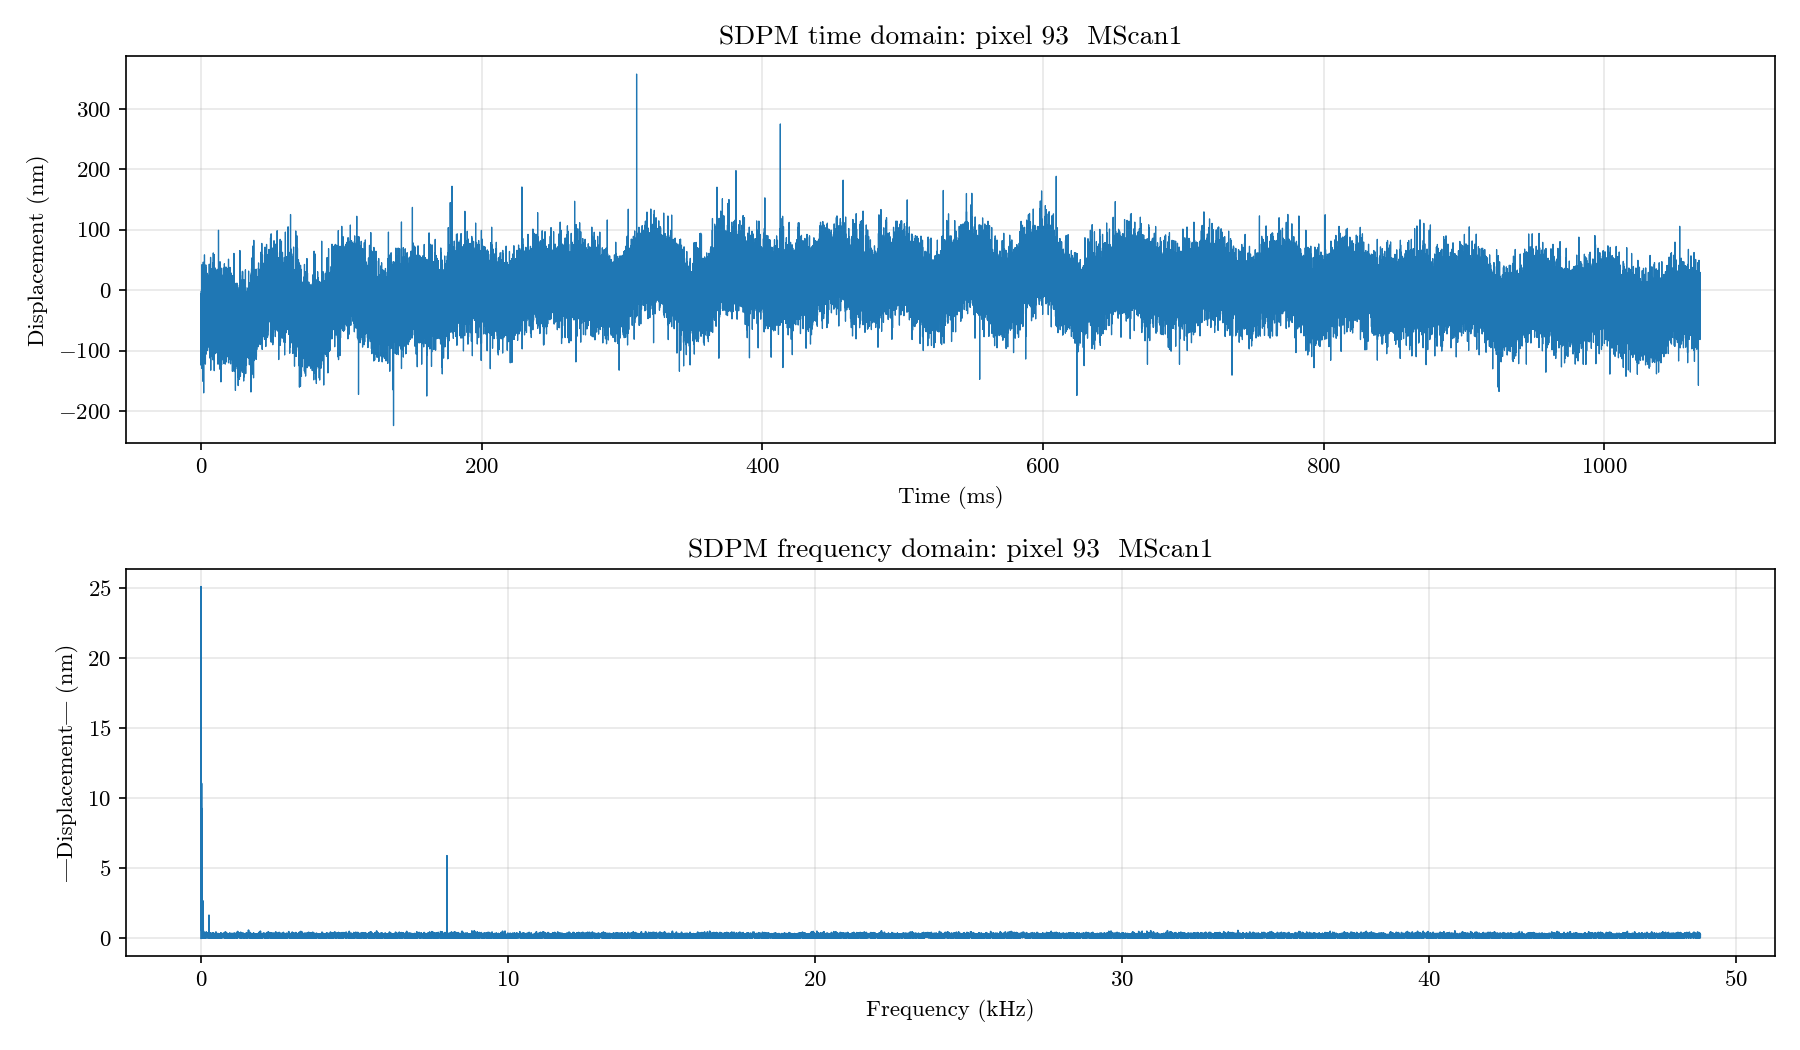
\includegraphics[width=\textwidth]{Results/mscan1_sdpm_pixelB.png}
  \caption{SDPM result for pixel B (index $93$, depth $0.335$~mm) in the single-tone M-scan. Top: displacement time series (nm). Bottom: one-sided displacement spectrum (nm).}
  \label{fig:mscan1_B}
\end{figure}

The time-domain signal at both pixels shows the envelope of a sinusoidal oscillation (though it is internally noisy). The zoomed time-domain view (Figure~\ref{fig:mscan1_zoom}) is very noisy, as expected, and unfortunately not interpretable, so we must rely on the frequency-domain analysis. 

The frequency-domain spectrum shows a single sharp peak at $8.011$~kHz for both pixels, identifying this as the tone played through the speaker. The displacement amplitudes at pixels A and B are $5.83$~nm and $5.90$~nm respectively, which are very close to each other, as expected given that both pixels are tracking the same membrane surface. The small difference in amplitude may be due to slight variations in the local reflectivity or noise, but overall the results are consistent with accurate SDPM tracking of the speaker membrane's vibration at the single tone frequency. The frequency-domain spectrum also show a very low noise floor, at the magnitude of sub-nanometer displacements, which is consistent with the high SNR of raw A-scans observed in previous sections.

It should be noted that the frequency-domain plots also display a large low-frequency and DC component, which is likely due to residual drift in the time-domain signal that was not fully removed by detrending, as well as transient artifacts at the beginning of the M-scan. These low-frequency components do not affect the identification of the tone frequency, which is well above this range.

\begin{figure}[ht]
  \centering
  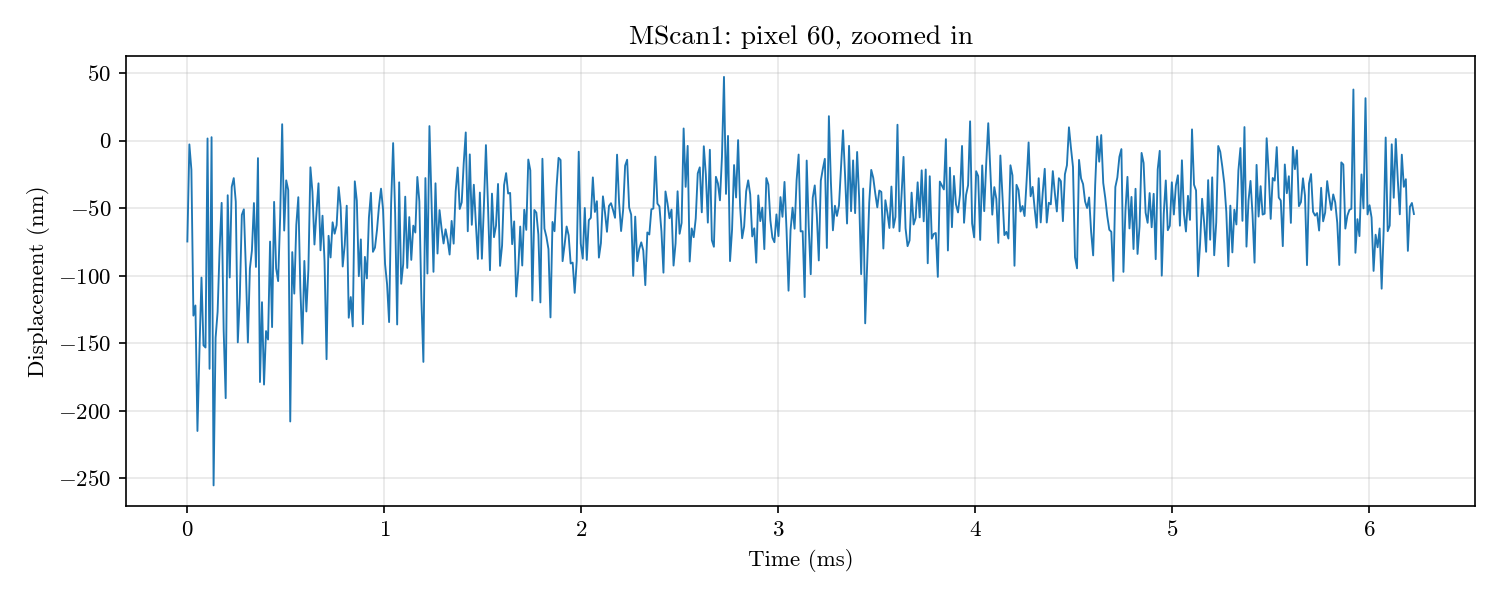
\includegraphics[width=0.8\textwidth]{Results/mscan1_zoom.png}
  \caption{Zoomed time-domain displacement at pixel A.}
  \label{fig:mscan1_zoom}
\end{figure}

\subsubsection{40-Tone M-Scan}


no distortions or harmonics, so approx linear speaker. but not all-pass.

\section{Conclusion}



% --- Bibliography ---
\printbibliography

\appendix
\counterwithin{figure}{section}
\counterwithin{table}{section}
\section{Background Scan Polynomial Fitting} \label{appendix:poly_fitting}
Figures~\ref{fig:poly_fit_bscan},~\ref{fig:poly_fit_mscan_1}, and~\ref{fig:poly_fit_mscan_40} show the averaged background spectrum and polynomial fit for the B-scan, single-tone M-scan, and 40-tone M-scan datasets, respectively. In all cases, a polynomial of degree $16$ was found to provide a good balance between smoothness and accuracy without introducing numerical instability.

\begin{figure}[ht]
  \centering
  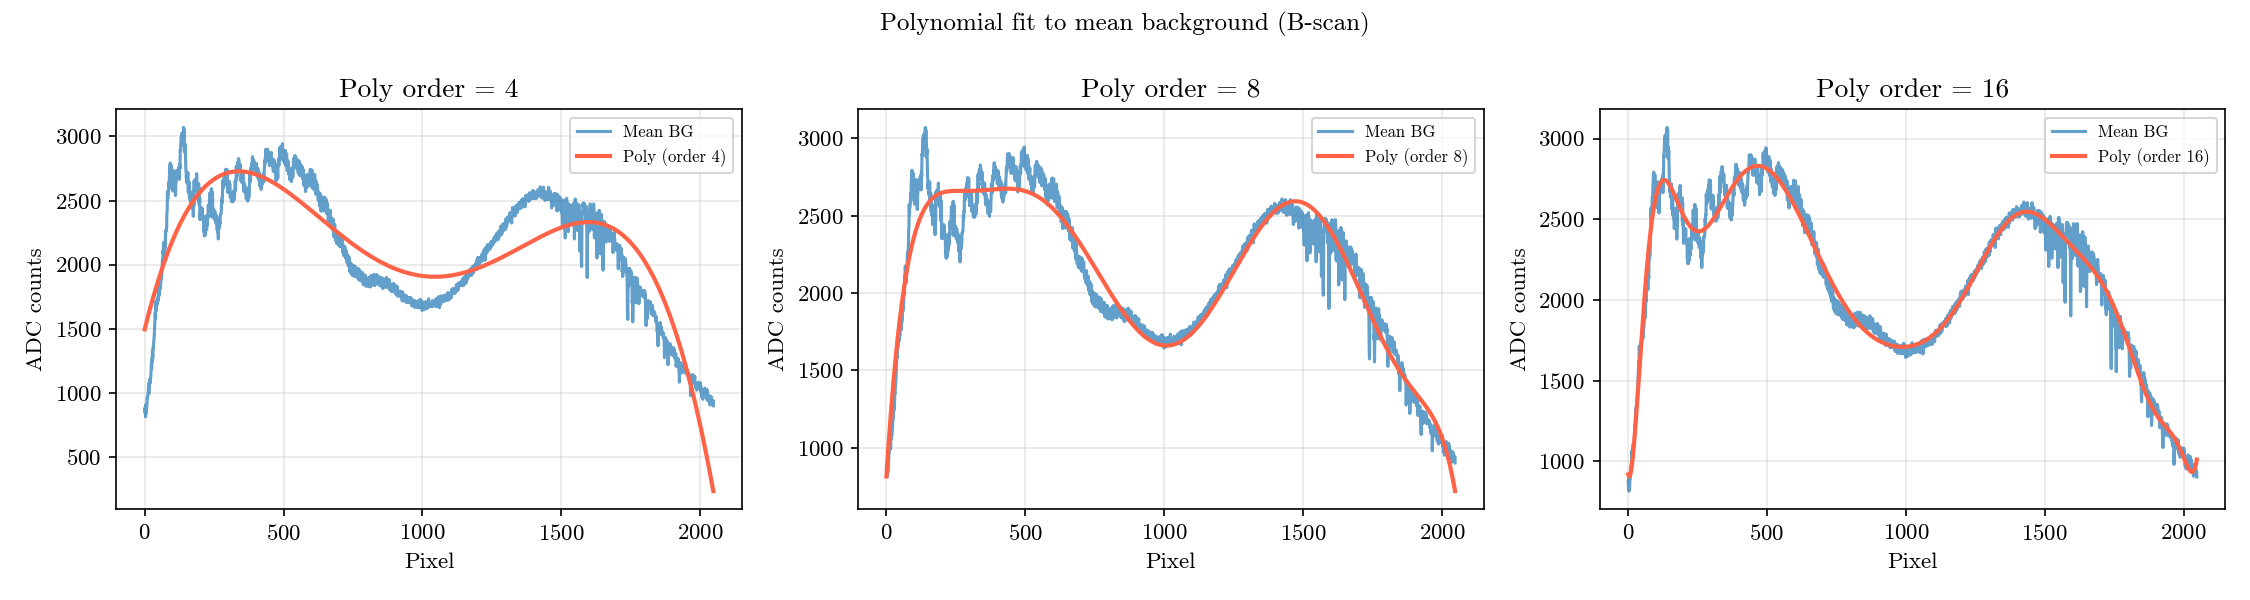
\includegraphics[width=\textwidth]{Results/poly_fit_comparison_bscan.png}
  \caption{Polynomial fitting of the averaged background spectrum for the B-scan dataset.}
  \label{fig:poly_fit_bscan}
\end{figure}

\begin{figure}[ht]
  \centering
  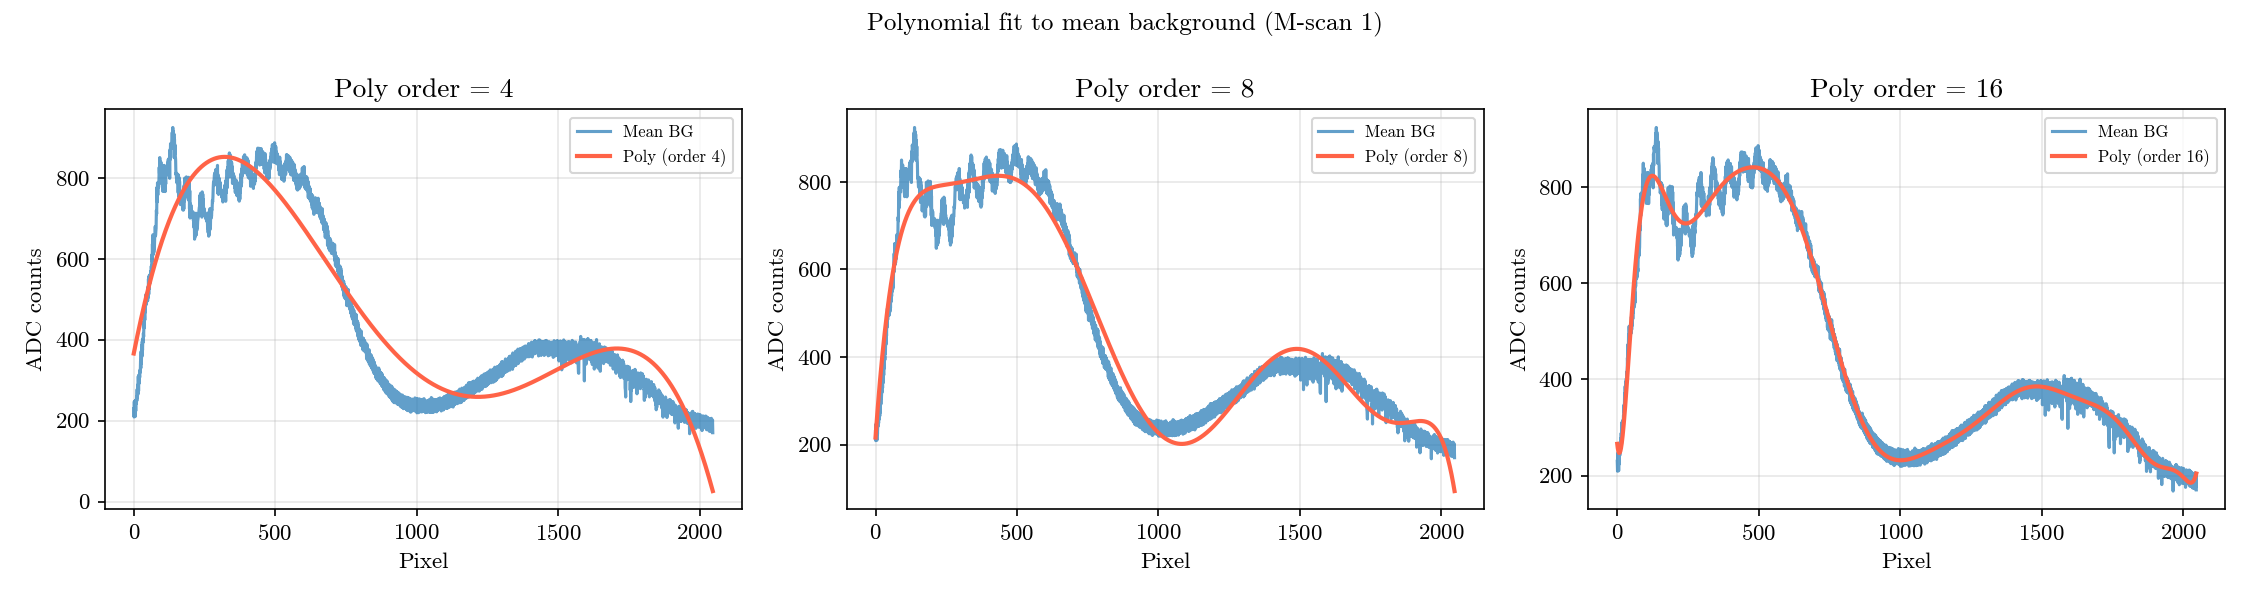
\includegraphics[width=\textwidth]{Results/poly_fit_comparison_mscan_1.png}
  \caption{Polynomial fitting of the averaged background spectrum for the single tone M-scan dataset.}
  \label{fig:poly_fit_mscan_1}
\end{figure}

\begin{figure}[ht]
  \centering
  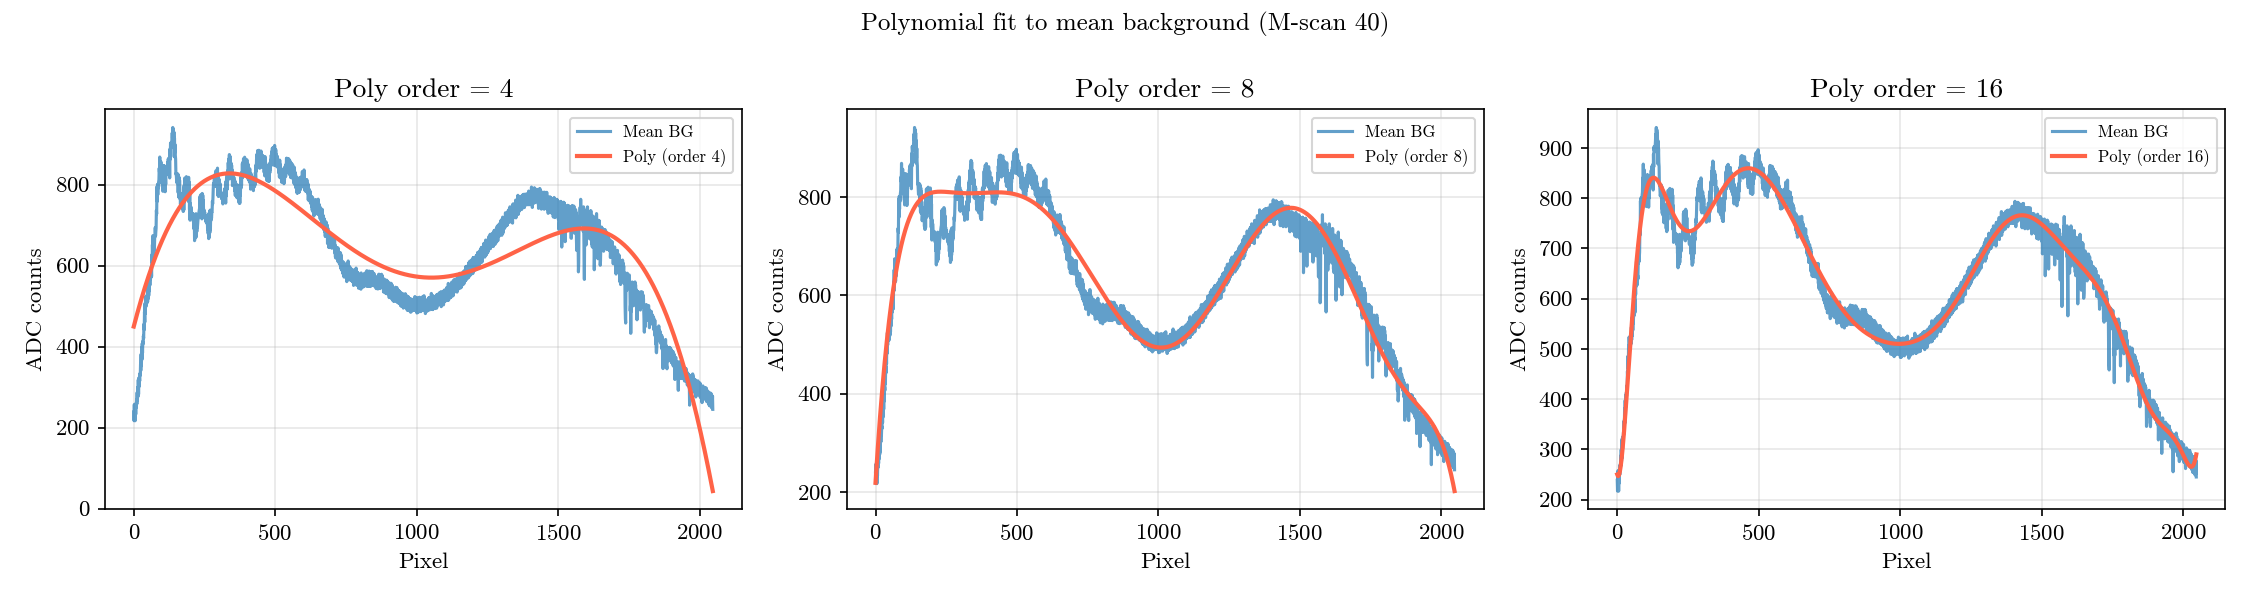
\includegraphics[width=\textwidth]{Results/poly_fit_comparison_mscan_40.png}
  \caption{Polynomial fitting of the averaged background spectrum for the 40-tone M-scan dataset.}
  \label{fig:poly_fit_mscan_40}
\end{figure}

\end{document}